\begin{frame}[parent={cmap:software-testing-foundations}, hasprev=false, hasnext=true]
\frametitle{Software testing}

\begin{block:fact}{Motivation}
\begin{itemize}
	\item Software contains fault.

	\item Testing the software can reveal several faults.
\end{itemize}
\end{block:fact}

\begin{block:fact}{Software testing as a discipline}
\begin{itemize}
	\item \textit{Ad hoc} testing is insufficient and ineffective at fault
	detection.
	\begin{itemize}
		\item It is hard to think of enough test cases even for simple software
		(such as \refie{example:triangle}{Triangle}).
	\end{itemize}

	\item Software testing must be taken as a discipline.
	\begin{itemize}
		\item Test cases must be designed to assess the quality of software
		artifacts (mainly the requirements specification and the source code)
		regarding given criteria.

		\item Techniques must be developed to detect as much faults as possible
		in the software.
	\end{itemize}
\end{itemize}
\end{block:fact}
\end{frame}


\begin{frame}[hasprev=true, hasnext=true]
\frametitle{Software testing}
\framesubtitle{Definition}
\label{concept:software-testing}

\begin{block:concept}{Definition}
Software testing is the process of operating a system or component under
specified conditions, observing or recording the results, and  making
an evaluation of some aspect of the system or component~\cite{ieee610.12:1990}.
\end{block:concept}

\begin{block:fact}{Software testing is\dots{}}
\begin{itemize}
	\item a verification and validation activity,

	\item important for maintenance, reliability assessment,software process
	improvement, debugging,

	\item a dynamic activity,
	\begin{itemize}
		\item It requires the execution of the program (static analysis is
		not enough),
	\end{itemize}

	\item expensive~\cite{harrold:2000}
\end{itemize}
\end{block:fact}
\end{frame}



\begin{frame}
\frametitle{Software testing}
\framesubtitle{Goal}

\begin{block:fact}{Goal}
\begin{itemize}
	\item The goal of software testing is to detect faults in the product
	under testing.
\end{itemize}
\end{block:fact}

\begin{block:fact}{}
First error ever detected (by Grace Hopper). It is an actual bug
(that is why we call errors of bugs till today).
\centering
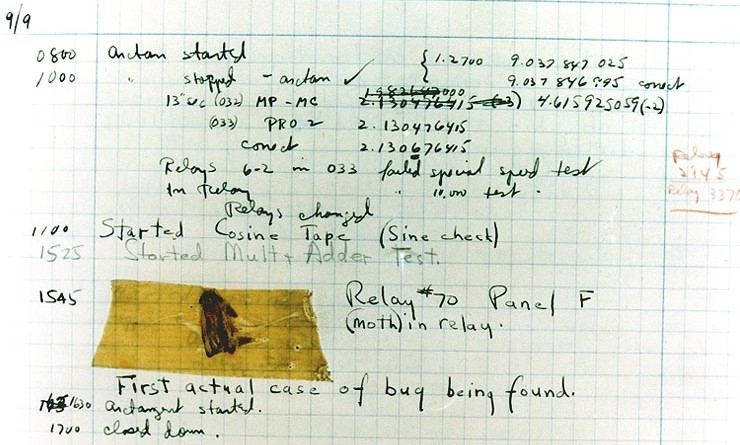
\includegraphics[width=7cm]{first-bug}
\end{block:fact}
\end{frame}


\begin{frame}
\frametitle{Software testing}
\framesubtitle{Rationale}

\begin{block:fact}{Contradiction}
\begin{itemize}
	\item Thus, software testing aims at virtually destroying the software?
	\begin{itemize}
		\item After all, the programmer spent hours implementing it and
		test activities will find errors in the work just done by him.
	\end{itemize}
\end{itemize}
\end{block:fact}

\begin{block:fact}{Rationale}
\begin{itemize}
	\item Humans are highly goal-oriented (and proper goals has an important
	psychological effect~\cite[p. 6]{myers:2004}).

	\item If the goal is to demonstrate that a program has no error, then the
	tester will subconsciously be steered toward this goal.
	\begin{itemize}
		\item There will be a tendency to select test data that have a low
		probability of causing the program to fail.
	\end{itemize}

	\item If the goal is to demonstrate that a program has error, the test data
	will have a higher probability of finding error.
\end{itemize}
\end{block:fact}
\end{frame}



\begin{frame}
\frametitle{Software testing}
\framesubtitle{Rationale}

\begin{block:principle}{Rationale}
The process of demonstrating that errors are not present is impossible to
achieve for virtually all programs (even trivial ones).
\end{block:principle}

\begin{block:fact}{Undecidable problems}
\begin{itemize}
	\item The assessment of the correctness of a program is an undecidable
	problem.
	\begin{itemize}
		\item Undecidable = non-computable.
	\end{itemize}

	\item Errors can be masked by other errors due to coincident correction.
	\begin{itemize}
		\item And assessment of coincident correct is also an undecidable
		problem.
	\end{itemize}

	\item Several other undecidable problems plague software testing: software
	equivalence, executability.
\end{itemize}
\end{block:fact}
\end{frame}


\begin{frame}
\frametitle{Sofware testing}
\framesubtitle{Main concepts}

\begin{block:fact}{How are faults detected?}
\begin{itemize}
	\item Faults are detected by running the software against a set of test
	cases.
\end{itemize}
\end{block:fact}

\begin{block:procedure}{Test case execution}
\begin{enumerate}
	\item Define the input data to be fed to the software under testing.

	\item Run the software.

	\item Check if the result the software produced was the expected one (for
	the given input data).
	\begin{itemize}
		\item If the result is correct, keep defining different input data.

		\item If the result is incorrect, a fault was found! Success!
	\end{itemize}
\end{enumerate}
\end{block:procedure}
\end{frame}



\begin{frame}
\frametitle{Sofware testing}
\framesubtitle{Main concepts}

\begin{block:principle}{Exhaustive testing}
If the software is executed against all possible input data,
any fault will be found!
\end{block:principle}

\begin{block:fact}{Feasibility and computability}
Unfortunately, it is often not possible to run exhaustive testing due to
some computational problems:
\begin{itemize}
	\item the input domain may be so big that it is impossible to run the
	software against it in a reasonable time,

	\item computability (undecidable problems).
\end{itemize}
\end{block:fact}
\end{frame}


\begin{frame}
\frametitle{Software testing}
\framesubtitle{Main concepts}

\begin{block:principle}{Domain partitioning}
Nonetheless, it is possible to partition the input domain and, instead of
using all elements within each partition, just a few ones are selected (and
accepted as a good representation of every element in the set).
\end{block:principle}

\begin{block:fact}{Techniques and criteria}
\begin{itemize}
	\item Test criterion defines rules regarding how a given input domain is
	partitioned.

	\item Such rules, when applied to the software under testing, generates
	test requirements.
	\begin{itemize}
		\item Test requirement is a combination of elements of the program
		under testing that must be satisfied by the execution of a test case.
	\end{itemize}

	\item Test technique defines the rationale and source of information that
	guides the development of test criteria.
\end{itemize}
\end{block:fact}
\end{frame}




\begin{frame}[c, hasprev=true, hasnext=false]
\frametitle{Software testing concepts}
\framesubtitle{Main concepts}

\begin{block:fact}{}
	\centering
	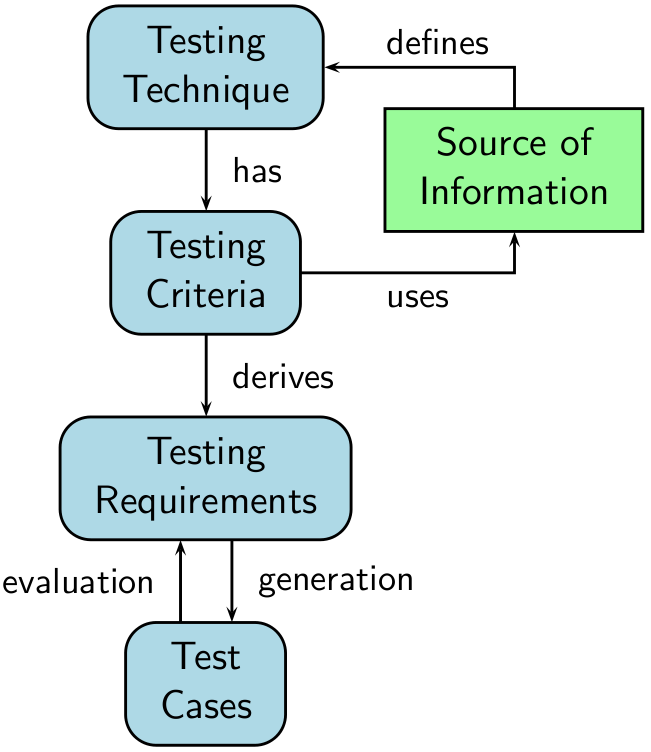
\includegraphics[scale=.3]{software-testing}
\end{block:fact}
\end{frame}